\documentclass[11pt]{amsart}

\usepackage[english]{babel}
\usepackage{appendix}
\usepackage{amsmath}
\usepackage{amsfonts}
\usepackage{amssymb}
\usepackage{showlabels}
\usepackage{hyperref}
\usepackage{amsthm}
\usepackage{marginnote}
\usepackage{stmaryrd}
\usepackage{enumitem}
\usepackage[english]{babel}
\usepackage{yfonts}
\usepackage[T1]{fontenc}
\usepackage[utf8x]{inputenc}
\usepackage{verbatim}
\usepackage{graphicx}
\usepackage{verbatim}
\usepackage{faktor}
\usepackage{xcolor}
\usepackage{xfrac}
\usepackage{tikz,tikz-cd}
\usetikzlibrary{decorations.pathmorphing,decorations.pathreplacing,patterns}

\usepackage[all]{xy}
\usepackage{bbm}
\usepackage{tabularx}
\usepackage{longtable}
\usepackage{tabu}
\usepackage{booktabs}
\usepackage{mathtools}

\usepackage[]{textcomp}
\usepackage[sups]{Baskervaldx}
\usepackage{cabin}
\usepackage[varqu,varl]{inconsolata}
\usepackage[baskervaldx,bigdelims,vvarbb]{newtxmath}
\usepackage[cal=cm]{mathalfa}


\newcommand{\plC}{\scalebox{0.8}[1.3]{$\sqsubset$}}

\newcommand{\TT}{\operatorname{T}}
\newcommand{\oM}{\overline{\mathcal{M}}}
\newcommand{\M}[4]{\overline{\mathcal{M}}_{#1,#2}(#3,#4)}
\newcommand{\Q}[4]{\mathcal{Q}_{#1,#2}(#3,#4)}
\newcommand{\Qe}[4]{\mathcal{Q}^{\epsilon}_{#1,#2}(#3,#4)}
\newcommand{\Qt}[4]{\widetilde{\mathcal Q}_{#1,#2}(#3,#4)}
\newcommand{\QG}[4]{\mathcal{Q}G_{#1,#2}(#3,#4)}
\newcommand{\QGe}[4]{\mathcal{Q}G^{\epsilon}_{#1,#2}(#3,#4)}
\newcommand{\D}[3]{\mathcal{D^Q}(#1,#2,#3)}
\newcommand{\E}[3]{\mathcal{E^Q}(#1,#2,#3)}
\newcommand{\PP}{\mathbb P}
\newcommand{\Z}{\mathbb{Z}}
\newcommand{\tVZc}[4]{\widetilde{\mathcal{V\!Z}}^{\rm{ctr}}_{#1,#2}(#3,#4)}
\newcommand{\VZc}[4]{\mathcal{V\!Z}^{\rm{ctr}}_{#1,#2}(#3,#4)}
\newcommand{\VZcLi}[4]{\mathcal{V\!Z}^{\rm{ctr, Li}}_{#1,#2}(#3,#4)}
\newcommand{\N}{\mathbb{N}}
\newcommand{\OO}{\mathcal{O}}
\renewcommand{\to}{\rightarrow}
\newcommand{\A}{\mathcal A}
\newcommand{\B}{\mathcal B}
\newcommand{\C}{\mathfrak C}
\newcommand{\cC}{\mathcal C}
\newcommand{\EE}{\mathbf{E}}
\renewcommand{\L}{\mathcal L}
\newcommand{\LL}{\mathbf{L}}
\newcommand{\MM}{\mathfrak M}
\newcommand{\Aaff}{\mathbb{A}}
\newcommand{\kfield}{\Bbbk}
\newcommand{\comp}{\chi}
\newcommand{\sst}{\sigma^{\operatorname{ss}}}
\newcommand{\Pic}{\operatorname{Pic}}
\newcommand{\Def}{\operatorname{Def}}
\newcommand{\Spec}{\operatorname{Spec}}
\newcommand{\Proj}{\operatorname{Proj}}
\newcommand{\Hom}{\operatorname{Hom}}
\newcommand{\Ext}{\operatorname{Ext}}
\newcommand{\Gm}{\mathbb{G}_{\text{m}}}
\newcommand{\virt}[1]{[#1]^{\operatorname{virt}}}
\newcommand{\vip}[1]{[#1]^{\operatorname{prod}}}
\newcommand{\Id}{\operatorname{Id}}
\newcommand{\CC}{\mathbb{C}}
\newcommand{\QQ}{\mathbb{Q}}
\newcommand{\HH}{\operatorname{H}}
\newcommand{\Achow}{\operatorname{A}}
\newcommand{\pt}{\operatorname{pt}}
\newcommand{\bq}{\begin{equation}}
\newcommand{\eq}{\end{equation}}
\newcommand{\ba}{\begin{aligned}}
\newcommand{\ea}{\end{aligned}}
\newcommand{\be}{\begin{enumerate}}
\newcommand{\ee}{\end{enumerate}}
\newcommand{\bsm}{\left(\begin{smallmatrix}}
\newcommand{\esm}{\end{smallmatrix}\right)}                   
\newcommand{\bpm}{\begin{pmatrix}}
\newcommand{\epm}{\end{pmatrix}}
\newcommand{\barr}{\begin{displaymath}\begin{array}{cccc}}
\newcommand{\earr}{\end{array}\end{displaymath}}
\newcommand{\barrl}{\begin{displaymath}\begin{array}{lcl}}
\newcommand{\earrl}{\end{array}\end{displaymath}}
\newcommand{\barl}{\begin{displaymath}\begin{array}{l}}
\newcommand{\earl}{\end{array}\end{displaymath}}
\newcommand{\bxym}{ \begin{displaymath}\xymatrix }
\newcommand{\exym}{\end{displaymath}}
\newcommand{\bcd}{\begin{center}\begin{tikzcd}}
\newcommand{\ecd}{\end{tikzcd}\end{center}}
\newcommand{\R}{\operatorname{R}^{\bullet}}
%\newcommand{\sslash}{\mathbin{/\mkern-6mu/}}
\newcommand{\tr}{{\rm tr}}
\newcommand{\Isom}{\text{Isom}}
\newcommand{\pr}{\operatorname{pr}}
\newcommand{\ev}{\operatorname{ev}}
\newcommand{\codim}{\operatorname{codim}}
\newcommand{\vdim}{\operatorname{vdim}}
\newcommand{\ildef}[1]{\emph{#1}}
\newcommand{\om}[1]{\mathcal{#1}}
\newcommand{\h}{\operatorname{h}}
\newcommand{\Aut}{\operatorname{Aut}}
\newcommand{\RR}{\textbf{R}}
\newcommand{\NN}{\operatorname{N}}


\theoremstyle{definition}
\newtheorem{thm}{Theorem}[section]
\newtheorem{lem}[thm]{Lemma}
\newtheorem{lemma}[thm]{Lemma}
\newtheorem{prop}[thm]{Proposition}
\newtheorem{cor}[thm]{Corollary}
\newtheorem*{teo*}{Theorem}
\newtheorem{ipotesi}{ipotesi}
\newtheorem*{nota}{Nota}
\newtheorem{claim}{Claim}
\newtheorem{question}[thm]{Question}
\newtheorem{conj}[thm]{Conjecture}

\newtheorem{innercustomthm}{Theorem}
\newenvironment{customthm}[1]
  {\renewcommand\theinnercustomthm{#1}\innercustomthm}
  {\endinnercustomthm}

\theoremstyle{definition}
\newtheorem{example}[thm]{Example}
\newtheorem{ex}[thm]{Example}
\newtheorem{dfn}[thm]{Definition}
\newtheorem{definition}[thm]{Definition}
\newtheorem{aside}[thm]{Aside}
\newtheorem{remark}[thm]{Remark}
\newtheorem{com}[thm]{Comment}
\newtheorem{num}{Number}
\newtheorem*{sketch}{Sketch}
\newtheorem*{rem}{Remark}
\newtheorem*{aside*}{Aside}
\newtheorem*{acknowledgements}{Acknowledgements}

\newcommand{\ilemph}[1]{\emph{#1}}

\setcounter{tocdepth}{2}

\newcommand{\todo}[1]{\vspace{5mm}\par \noindent
\framebox{\begin{minipage}[c]{0.95 \textwidth} \tt #1\end{minipage}} \vspace{5mm} \par}

\def\ti{-\allowhyphens}
\newcommand{\thismonth}{\ifcase\month % case 0 --- impossible!
  \or January\or February\or March\or April\or May\or June%
  \or July\or August\or September\or October\or November%
  \or December\fi}
\newcommand{\thismonthyear}{{\thismonth} {\number\year}}
\newcommand{\thisdaymonthyear}{{\number\day} {\thismonth} {\number\year}}

\title[Genus One Reduced Relative Invariants]{Relative Stable Maps in Genus One via Central Alignments}
\author{Luca Battistella, Navid Nabijou and Dhruv Ranganathan}
\date{\thismonthyear}

\begin{document}


\begin{abstract} For a smooth projective variety $X$ and a smooth very ample hypersurface $Y \subseteq X$, we define moduli spaces of relative stable maps to $(X,Y)$ in genus one, as closed substacks of the moduli space of maps from centrally aligned curves, constructed in \cite{RSPW}. We construct virtual classes for these moduli spaces, which we use to define \emph{reduced relative Gromov--Witten invariants} in genus one.

[GOALS: We prove a recursion formula which allows us to completely determine these invariants in terms of the reduced Gromov--Witten invariants, as defined in [REF]. We also prove a relative version of the Li--Zinger formula, relating our invariants to the usual relative Gromov--Witten invariants. Also say something about quasimaps.]
\end{abstract}

\maketitle

\appendixtitletocoff
\tableofcontents

\section{The space of relative centrally aligned maps}
\noindent Recall \cite{RSPW} that the moduli space of maps from centrally aligned curves is obtained by first considering the  Cartesian diagram
\bcd
\tVZc{1}{n}{X}{\beta}\ar[d]\ar[r]\ar[dr,phantom,"\Box"] & \M{1}{n}{X}{\beta}\ar[d] \\
\MM_{1,n}^{\rm{ctr}}\ar[r] & \MM_{1,n}^{\dagger}
\ecd
so that objects of $\tVZc{1}{n}{X}{\beta}$ consist of
\begin{enumerate}
\item a centrally aligned curve $(C,M_C,\delta)$;
\item a stable map $f\colon C \to X$;
\end{enumerate}
subject to the condition that the contraction radius $\delta$ of the central alignment is equal to $\delta_f$, the contraction radius of the stable map $f$. We then define
\begin{equation*} \VZc{1}{n}{X}{\beta} \subseteq \tVZc{1}{n}{X}{\beta} \end{equation*}
to be the closed substack consisting of maps satisfying the \emph{factorisation condition}, namely that the map $f\colon C\to X$ factors through the associated contraction to a Smyth curve, i.e. there exists a map $\bar{f}$ making the following square commute:
\bcd
\widetilde C\ar[r]\ar[d] & \overline C\ar[d,"\bar f" left,dotted] \\
C\ar[r,"f"] & X
\ecd
One should think of the factorisation condition as identifying the main component of the moduli space.

\subsection{Definition of the relative space} We now give the central definition of this article.
\begin{dfn}
Fix a vector of tangency conditions $\alpha=(\alpha_1,\ldots,\alpha_n)$ with $\Sigma_{i=1}^n \alpha_i \leq Y \cdot \beta$. Then the \emph{centrally aligned relative space} 
\begin{equation*}\VZc{1}{\alpha}{X|Y}{\beta} \end{equation*}
is defined to be the closed substack of $\VZc{1}{n}{X}{\beta}$ satisfying the following conditions:
\begin{enumerate}
\item \emph{Gathmann's relative condition:} for each connected component $Z$ of $f^{-1}(Y)$, either:
\begin{enumerate}
\item $Z$ is a single point of $C$, in which case if $Z=x_i$ is a marking then we require that the multiplicity of $f$ at $x_i$ along $Y$ is at least $\alpha_i$ (if $Z$ is not a marking then there is no condition);
\item $Z$ is a subcurve $Z \subseteq C$, in which case we require that
\begin{equation*} f^*[Y]|_Z -\sum_{x_i\in Z}\alpha_ix_i\end{equation*}
is an effective class in $\Achow_0(Z)$. Since $Z$ is at most genus one and any line bundle of strictly positive degree on a Gorenstein genus one curve is effective, this condition can be rephrased as the following numerical criterion
\begin{equation*} Y \cdot f_*[Z]+\sum_{j=1}^r m_j\geq \sum_{x_i\in Z}\alpha_i \end{equation*}
where the $m_j$ denote the multiplicities of $f$ along $Y$ at the points $y_j \in Z \cap \overline{C \setminus Z}$ (necessarily a finite number of nodes), together with the requirement that, when we have equality in the above, there is an isomorphism of line bundles:
\begin{equation*} (f|_{Z})^*\OO_X(Y) \otimes \OO_Z\left(\sum_{j=1}^r m_j y_j\right)=\OO_Z\left(\sum_{x_i\in Z}\alpha_ix_i\right)\end{equation*}
\end{enumerate}

\item \emph{Novel condition:} if $v_1,v_2$ are two vertices belonging to $R_\delta$, then the corresponding tangencies to the divisor $m_{j_1}$ and $m_{j_2}$ must be equal. Here $R_\delta$ is the set of vertices $v \in \plC$ with $\lambda(v)=\delta$ equal to the contraction radius.
\end{enumerate}
\end{dfn}

\begin{remark}
Trying to straighten out Gathmann's condition for a curve component of $f^{-1}(Y)$ into an easily verifiable criterion: if $Z$ is a smooth elliptic curve, recall that every line bundle of positive degree on it is effective, hence the relative condition can be rephrased as the following numerical criterion:
\begin{equation*} f_*[Z]\cdot [Y]+\sum_{j=1}^r m^{(j)}\geq \sum_{x_i\in Z}\alpha_i \end{equation*}
together with the additional requirement that, when the above is an equality, there is an isomorphism of line bundles:
\begin{equation}\label{eqn:eq_in_Pic}
(f|_{Z})^*\OO_X(Y) \otimes \OO_Z\left(\sum_{j=1}^r m^{(j)}y_j\right)=\OO_Z\left(\sum_{x_i\in Z}\alpha_ix_i\right) 
\end{equation}
 
 If $Z$ is reducible, the correct extension is not to impose the same condition componentwise; rather, we should ask the numerical condition for the total degree, and, if $Z$ is obtained by gluing a smooth elliptic curve $E$ with a forest of rational trees $R_i$ at roots $q^E_i$, then the line bundle equality \eqref{eqn:eq_in_Pic} should be required in $\Pic(E)$ after counting each $q^E_i$ towards the left hand side with multiplicity
 \[f_*[R_i]\cdot [Y]+\sum_{\text{external components attached to $R_i$}} m^{(j)}- \sum_{x_j\in R_i}\alpha_j.\]
 
 That this is the right thing to do follows from the proof that Gathmann's relative space is the projection of Jun Li's moduli space of maps to the expanded pair after contracting the higher levels of the accordion.
\end{remark}

\section{The relative space is equal to the closure of the nice locus for $(\PP^N,H)$}
\noindent In general we do not know very much about the space we have just defined. The aim of this section is to show that, in the case where $X=\PP^N$ and $Y=H$ is a hyperplane, the space is proper and irreducible of the expected dimension. As such it has a fundamental class, which we can use to define reduced relative Gromov--Witten invariants in genus one.

\begin{remark} In the case of a general pair $(X,Y)$ we will see that the moduli space is still proper, but is not in general irreducible or even equidimensional. Nevertheless, we can equip it with a virtual class by `pulling back'' from the case of $(\PP^N,H)$; for details, see \S [REF]. \end{remark}

The strategy is as follows. We define (Definition \ref{Definition of nice locus})an open subspace
\begin{equation*}\VZc{1}{\alpha}{\PP^N|H}{d}^{\circ} \subseteq \VZc{1}{\alpha}{\PP^N|H}{d}\end{equation*}
called the \emph{nice locus}, on which the source curve and the map take a particularly simple form. Because of this simplicity, it is easy to show that the nice locus is irreducible (Lemma \ref{Nice locus is irreducible}). We then prove that $\VZc{1}{\alpha}{\PP^N|H}{d}$ is equal to the closure of the nice locus inside $\VZc{1}{n}{\PP^N}{d}$. Thus it is proper, since it is a closed space of a proper space, and it is irreducible, since it is the closure of an irreducible space inside an irreducible space.

\begin{definition} \label{Definition of nice locus} The \emph{nice locus} is defined as the open substack
\begin{equation*}\VZc{1}{\alpha}{\PP^N|H}{d}^{\circ} \subseteq \VZc{1}{\alpha}{\PP^N|H}{d}\end{equation*}
of centrally aligned maps satisfying the following two conditions:
\begin{enumerate}
\item the source curve $C$ is irreducible;
\item $f$ does not map $C$ inside $H$.
\end{enumerate}
\end{definition}

\begin{lem}\label{Nice locus is irreducible}
The nice locus $\VZc{1}{\alpha}{\PP^N|H}{d}^{\circ}$ is irreducible.
\end{lem}
\begin{proof}
By definition the contraction radius $\delta$ is compatible with the map, i.e. the subcurve $C_0\subseteq C$ where $\lambda<\delta$ is equal to the maximal connected genus one subcurve contracted by $f$. Hence when the source curve is irreducible we must have $\delta=0$, and we see that the central alignment on $C$ is uniquely and trivially determined. Thus to specify a point in the nice locus we only need to specify the source curve $C$ (as a scheme) and the map $f$. A parametrisation can be given from the vector bundle:\marginnote{I'm sure there's a simpler way to say this - Navid}
\[ \operatorname{Vb}\left(\pi_*\OO_{\mathcal E}(\sum_{j=n+1}^{n+\delta}\sigma_j)\oplus\pi_*\OO_{\mathcal E}(\sum_{j=1}^{n+\delta}\sigma_j)^{\oplus r}\right) \quad \text{on} \quad \mathcal{M}_{1,n+\delta}\]
where $\pi\colon\mathcal E\to\mathcal M$ is the universal curve and $\delta=d-\sum\alpha_i$.
\end{proof}

\subsection{Justifying the novel condition}
Remember that we are trying to impose conditions which determine the closure of the nice locus inside the moduli space of centrally aligned maps. Here is one example where we show by a dimensional computation that the novel condition must be included if we hope to determine the closure of the nice locus.
\begin{example}
Consider $\M{1}{(3)}{\PP^1|H}{3}$. The virtual dimension is $7-3=4$. Here is a parametrisation of the nice locus: choose an element $(E,p)$ of $\oM_{1,1}\setminus\partial\oM_{1,1}$ (which has dimension $1$), and let $s_0$ be the natural section $s_0 \colon\OO_E\hookrightarrow\OO_E(3p)$ and $s_1$ any other section of $\OO_E(3p)$ not vanishing at $p$ (notice that $\h^0(E,\OO_E(3p))=3$). Then $(E,p,[\lambda s_0,s_1])$ gives a well-defined element of the nice locus for $\lambda \neq 0$.

Consider now the following weighted graph for a map in the boundary
\begin{center}
\begin{tikzpicture}
\draw[color=brown] (0,0) node[left]{$E$} -- (4,0);
\draw[fill=black] (1,0) circle[radius=2pt] node[above]{$x_1$};
\draw[fill=black] (2,0) circle[radius=2pt] node[below right]{$y_1$};
\draw[fill=black] (3,0) circle[radius=2pt] node[below right]{$y_2$};
\draw (2,1.5) node[left]{$R_1$} (3,1.5) node[left]{$R_2$};
\draw (2,-1) -- (2,2) node[above]{$2$} (3,-1) -- (3,2) node[above]{$1$};
\draw[->] (5,0.5) -- (8,0.5);
\draw (9,-1) -- (9,2) node[above]{$\PP^1$};
\draw[fill=black] (9,0) circle[radius=2pt] node[right]{$H$};
\end{tikzpicture}
\end{center}
where the brown line represents a contracted genus $1$ curve. Now $(E,x_1,y_1,y_2)$ is a point of $\oM_{1,3}$ subject to the divisorial condition $3x_1-2y_1-y_2=0\in \Achow_0(E)$; furthermore we have to choose the second branch point of the $2\colon 1$ map from $R_1$ to $\PP^1$. This already makes up for a $3$-dimensional moduli space of degenerate relative maps corresponding to such a graph. The minimal log structure for this curve has a chart from $\mathbb N^2$, with generators $e_1$ and $e_2$ corresponding to the smoothing parameters of the two nodes. If we allowed $e_1$ and $e_2$ to be identified in the characteristic sheaf, then we would get an extra $\Gm$ of choices for the log structure, so in total a $4$-dimensional moduli space. Thus if we don't impose the novel condition then we get a whole other component of the relative space, which of course for dimensional reasons cannot be contained in the closure of the nice locus.
\end{example}

\begin{remark}
 For the non-expert reader, it might be convenient to recall that the extra data of a centrally aligned log structure on the curves gives a modular interpretation to the iterated blow-up procedure of Vakil and Zinger. In particular the novel condition on the log structure can be translated into a closed condition on the exceptional loci of these blow-ups. 
\end{remark}

\begin{example} In this example we will give further moral justification for the novel condition, using as motivation the expanded degenerations approach to relative stable maps. This is not strictly necessary for what we want to do (since our spaces don't involve expanded degenerations), but it helps to explain where this condition comes from.

So, let us pretend that we have a good definition of the ``centrally aligned Li space'' of maps from centrally aligned curves to expanded degenerations:
\begin{equation*} \VZcLi{1}{\alpha}{X|D}{\beta} \end{equation*}
Objects of this moduli space should consist of maps $C \to \mathfrak{X}$ where $\mathfrak{X} \to X$ is an expansion of the pair $(X,D)$, together with a central alignment on $C$ which is compatible with this map. The factorisation property should say that the following diagram commutes:
\bcd
& \tilde{C} \ar[ld,"\nu" left] \ar[rd,"\tau"] & \\
C \ar[d,"f" left] & & \overline{C} \ar[d,"\overline{f}", dotted] \\
\mathfrak{X} \ar[rd,"\pi"] & & \mathfrak{X} \ar[ld,"\pi"] \\
& X & 
\ecd
Morally speaking, the projection map
\begin{equation*} \pi_* \colon \VZcLi{1}{\alpha}{X|D}{\beta} \to \VZc{1}{n}{X}{\beta} \end{equation*}
should have as its image our space $\VZc{1}{\alpha}{X|D}{\beta}$. We will see that everything in the image of this space must satisfy the novel condition, thus providing further justification for us imposing it.

We proceed by contradiction. Consider a genus one map $C \to \PP^1$ of the following form
\begin{center}
\begin{tikzpicture}
\draw[fill=black] (0,0) node[left]{$E$} -- (4,0);
\draw[fill=black] (0.7,0) circle[radius=2pt] node[below]{$5$};
\draw[fill=black] (2,0) circle[radius=2pt] node[above right]{$2$};
\draw[fill=black] (3,0) circle[radius=2pt] node[above right]{$3$};
\draw (2,1.5) node[right]{$C_1$};
\draw (3,1.5) node[right]{$C_2$};
\draw (2,-1) -- (2,2) node[above]{$2$};
\draw (3,-1) -- (3,2) node[above]{$3$};

\draw[->] (4.5,0) -- (6.5,0);
\draw (5.5,0) node[above]{$f$};
\draw (7,-1) -- (7,2) node[above]{$\PP^1$};
\draw[fill=black] (7,0) circle[radius=2pt] node[right]{$\infty$};
\end{tikzpicture}
\end{center}
and equip the source curve $C$ with a central alignment which identifies the lengths of the components $C_1$ and $C_2$:
\begin{center}
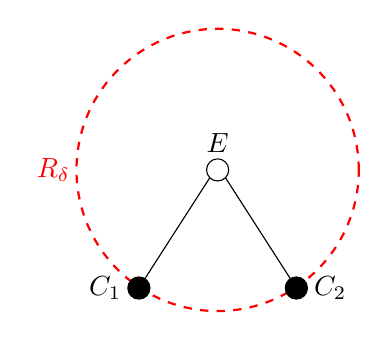
\begin{tikzpicture}
\draw[red,thick,dashed] (0,0) circle[radius=51pt];
\draw[red] (-1.75,0) node[left]{$R_\delta$};
\draw[fill=white] (0,0) circle[radius=4pt];
\draw (0,0.1) node[above]{$E$};
\draw[fill=black] (-1,-1.5) circle[radius=4pt];
\draw (-1.1,-1.5) node[left]{$C_1$};
\draw[fill=black] (-0.1,-0.1) -- (-1,-1.5);
\draw[fill=black] (1,-1.5) circle[radius=4pt];
\draw (1.1,-1.5) node[right]{$C_2$};
\draw[fill=black] (0.1,-0.1) -- (1,-1.5);
\end{tikzpicture}
\end{center}
This defines an ``object'' of $\VZc{1}{(5)}{\PP^1|\infty}{5}$, satisfying all the necessary conditions \emph{except for the novel condition}. We will show that this cannot belong to the image of $\pi_*$.

First we have to identify what the possible lifts of this object to the centrally aligned Li space are. The map $C \to \mathfrak{X}$ takes the following form:

\begin{center}
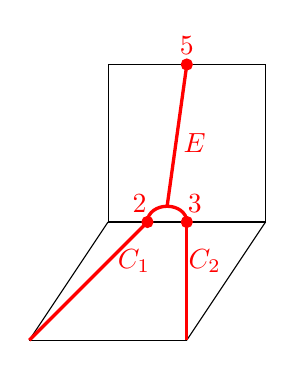
\begin{tikzpicture}
\draw (-1,-1) -- (1,-1);
\draw (-1,-1) -- (-1,1);
\draw (1,-1) -- (1,1);
\draw (-1,1) -- (1,1);
\draw (-1,-1) -- (-2,-2.5);
\draw (-2,-2.5) -- (0,-2.5);
\draw (0,-2.5) -- (1,-1);
\draw[red,very thick] (-2,-2.5) -- (-0.5,-1);
\draw[red] (-1,-1.5) node[right]{$C_1$};
\draw[red,fill=red] (-0.5,-1) circle[radius=2pt];
\draw[red] (-0.6,-1) node[above]{$2$};

\draw[red,very thick] (0,-2.5) -- (0,-1);
\draw[red] (-0.1,-1.5) node[right]{$C_2$};
\draw[red,fill=red] (0,-1) circle[radius=2pt];
\draw[red] (0.1,-1) node[above]{$3$};

\draw[red,very thick] (-0.5,-1) to [out=90,in=180] (-0.25,-0.8) to [out=0,in=90] (0,-1);
\draw[red,very thick] (-0.25,-0.8) -- (0,1);
\draw[red] (0.1,0) node{$E$};
\draw[red,fill=red] (0,1) circle[radius=2pt] node[above]{$5$};
\end{tikzpicture}
\end{center}
(Here the box at level $1$ represents a single fibre of the expanded degeneration; $E$ is mapped into a fibre and has zero horizontal degree.) In this case $\tilde{C}$ is obtained from $C$ by bubbling a rational component at the marking, and so the map $\tilde{C} \to \mathfrak{X}$ is given by:

\begin{center}
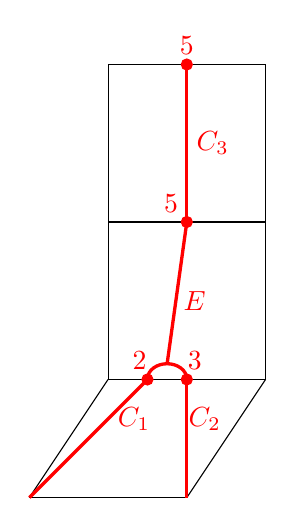
\begin{tikzpicture}
\draw (-1,-1) -- (1,-1);
\draw (-1,-1) -- (-1,1);
\draw (1,-1) -- (1,1);
\draw (-1,1) -- (1,1);
\draw (-1,-1) -- (-2,-2.5);
\draw (-2,-2.5) -- (0,-2.5);
\draw (0,-2.5) -- (1,-1);
\draw (-1,1) -- (-1,3);
\draw (-1,3) -- (1,3);
\draw (1,3) -- (1,1);
\draw[red,very thick] (-2,-2.5) -- (-0.5,-1);
\draw[red] (-1,-1.5) node[right]{$C_1$};
\draw[red,fill=red] (-0.5,-1) circle[radius=2pt];
\draw[red] (-0.6,-1) node[above]{$2$};

\draw[red,very thick] (0,-2.5) -- (0,-1);
\draw[red] (-0.1,-1.5) node[right]{$C_2$};
\draw[red,fill=red] (0,-1) circle[radius=2pt];
\draw[red] (0.1,-1) node[above]{$3$};

\draw[red,very thick] (-0.5,-1) to [out=90,in=180] (-0.25,-0.8) to [out=0,in=90] (0,-1);
\draw[red,very thick] (-0.25,-0.8) -- (0,1);
\draw[red] (0.1,0) node{$E$};
\draw[red,fill=red] (0,1) circle[radius=2pt];
\draw[red] (-0.2,1) node[above]{$5$};

\draw[red, very thick] (0,1) -- (0,3);
\draw[red] (0,2) node[right]{$C_3$};
\draw[red,fill=red] (0,3) circle[radius=2pt] node[above]{$5$};
\end{tikzpicture}
\end{center}

\end{example}

\subsection{Proof}
We now want to show that the relative space in the centrally aligned setting is equal to the closure of the nice locus; irreducibility then follows immediately. We start with one direction.

\begin{lem}
The closure of the nice locus is contained in the relative space.
\end{lem}
\begin{proof}
We address the relative conditions one at a time. Notice that they are all obviously satisfied on the nice locus.

The factorisation property is closed: see \cite[Theorem 4.3]{RSPW}.

Gathmann's relative condition is closed: see \cite[Proposition 4.9]{Vre}.

It remains to show that the novel condition is satisfied on the closure of the nice locus. Here is no proof but rather some heuristics. Consider for example a map similar to the one above
\begin{center}
\begin{tikzpicture}
\draw[color=brown] (0,0) node[left]{$E$} -- (4,0);
\draw[fill=black] (1,0) circle[radius=2pt] node[above]{$x_1$};
\draw[fill=black] (2,0) circle[radius=2pt] node[below right]{$y_1$};
\draw[fill=black] (3,0) circle[radius=2pt] node[below right]{$y_2$};
\draw (2,1.5) node[left]{$R_1$} (3,1.5) node[left]{$R_2$};
\draw (2,-1) -- (2,2) node[above]{$3$} (3,-1) -- (3,2) node[above]{$2$};
\draw[->] (5,0.5) -- (8,0.5);
\draw (9,-1) -- (9,2) node[above]{$\PP^1$};
\draw[fill=black] (9,0) circle[radius=2pt] node[right]{$H$};
\draw[fill=black] (9,1.5) circle[radius=2pt] node[right]{$H'$};
\end{tikzpicture}
\end{center}
and assume that it is in the closure of the nice locus; I want to argue that the two smoothing parameters cannot be identified. By the previous points I may assume that the factorisation property and Gathmann's relative conditions hold. I have a diagram:
\bcd
\cC^{\rm{ss}}\ar[r]\ar[dr] & \widetilde \cC\ar[r]\ar[d] & \overline \cC\ar[d,"\bar f"] \\
& \cC\ar[r,"f"] & X
\ecd
where I have included the semistable model of $\cC$ (and $\widetilde \cC$), thought of as a curve marked with $f^{-1}(H')$ as well, where $H\neq H'\in\PP^1$.

Notice that $\cC$ is a normal surface with at worst singular points at the nodes of $C=\cC_0$ (the central fibre $C=E+R_1+R_2$ is Cartier and a variety is smooth at any smooth point of a Cartier divisor) and the singularities are of type $A_{n_i},\ i=1,2$ (from the deformation theory of nodal curves).

I assume maximal multiplicity $\sum\alpha=d$, i.e. I am looking at the moduli space $\M{1}{(5)}{\PP^1|H}{5}$. Hence the line bundle and $s_0$ are determined as $f^*\OO_{\PP^1}(1)=\OO_{\cC}(5x_1)\otimes\OO_{\cC}(\beta E)$ for some (positive rational) $\beta$ and $s_0$ is the natural inclusion of $\OO_{\cC}$ (up to $\Gm$). 

The map is totally ramified at $y_i$ by Gathmann's condition. We conclude:
\[ \frac{\beta}{n_i+1}=(\beta E)\cdot R_i=m^{(i)}\]
Hence, having fixed the multiplicities, the two possible singularities of $\cC$ determine each other. In our example we may pick $n_1=1,\ n_2=2,\ \beta=6$. But knowing the singularity determines the semistable model: in our case $y_1$ is replaced by a $(-2)$-curve and $y_2$ by a chain of two $(-2)$-curves. Now we know from the work of Smyth \cite[Proposition 2.12]{SMY1} that the exceptional locus of $\cC^{\rm{ss}}\to\overline\cC$ is balanced, therefore we may deduce that $\bar f$ is constant on the branch of the genus $1$ singularity to which $R_2$ is joined, so $\overline C$ looks like this:

\begin{center}
\begin{tikzpicture}
\draw (-1,0) -- (1,0) node[right]{$\overline R_1$};
\draw[color=gray!50] (-1,-1) -- (1,1);
\draw[fill=black] (-.75,-.75) circle[radius=2pt] node[left]{$x_1$};
\draw[color=gray!50] (0,-1) -- (0,1);
\draw (-1,1.5) node[above left]{$\overline R_2$} -- (.25,.5);
\end{tikzpicture}
\end{center}
where a gray line is contracted by the map. On the other hand if $\delta=\lambda(v_1)=\lambda(v_2)$ then the prescription of \cite[Proposition 3.6.1]{RSPW} implies that $\tilde C\to \overline C$ looks like:
\begin{center}
\begin{tikzpicture}
\draw[color=brown] (0,0) node[left]{$E$} -- (4,0);
\draw[color=gray!50] (1,-1) -- (1,2);
\draw[fill=black] (1,1) circle[radius=2pt] node[left]{$x_1$};
\draw (2,1.5) node[left]{$R_1$} (3,1.5) node[left]{$R_2$};
\draw (2,-1) -- (2,2) node[above]{$3$} (3,-1) -- (3,2) node[above]{$2$};
\draw[->] (5,0.5) -- (7,0.5);
\draw (8,0.5) -- (10,0.5) node[right]{$\overline R_1$};
\draw[color=gray!50] (8,-.5) -- (10,1.5);
\draw[fill=black] (8.25,-.25) circle[radius=2pt] node[left]{$x_1$};
\draw (9,-.5) -- (9,1.5) node[above left]{$\overline R_2$};
\end{tikzpicture}
\end{center}
which is a contradiction.
\end{proof}

It thus remains to show that, given a relative radially aligned map, we can smooth it to one in the nice locus. \textcolor{red}{This is done by considering different cases locally, then gluing. \marginpar{What do we exactly mean by this? How does gluing work in the centrally aligned setting?}}

\subsection*{Case 1: non-contracted genus one internal component} Assume that the curve takes the form
\begin{equation*} C = C_0 \cup C_1 \cup \ldots \cup C_k \end{equation*}
where all the $C_i$ are smooth, $C_0$ has genus one, all the other $C_i$ have genus zero, and for $i \in \{1,\ldots,k\}$, $C_i$ intersects $C_0$ at a single node (denoted $q_i$) and does not intersect any other components.

Suppose furthermore that $C_0$ is a non-contracted \emph{internal component}, meaning that it is mapped into $H$ via $f$, and that $C_1$,\ldots,$C_k$ are \emph{external components}, meaning that they are not mapped into $H$ via $f$. The picture is:

[FIGURE]

Suppose that this is a relative stable map. This means that [BLAH]. We claim that it can be smoothed to a relative stable map in the nice locus. The construction depends on choosing an appropriate smoothing of the curve $C$, so that the map also smooths.

We start with $W = C_0 \times \Aaff^1_t$ (where $t$ denotes a fixed co-ordinate on the affine line). This is a smooth surface, fibred over $\Aaff^1_t$, with fibre equal to the elliptic curve $C_0$. Consider the points $q_1, \ldots, q_k$ on $C_0$. We will perform a series of weighted blow-ups at the points $(q_i,0) \in W$, in order to obtain a surface whose general fibre is smooth (in fact, isomorphic to $C_0$) and whose central fibre is isomorphic to $C$.

Fix $i \in \{1,\ldots,k\}$ and let $m_i$ be the multiplicity of $f$ with $H$ at $q_i \in C_i$. We define:
\begin{equation*} l = \operatorname{lcm}(m_1,\ldots,m_k) \qquad r_i = l/m_i \end{equation*}
We now blow-up the surface $W$ at the points $(q_i,0)$ with weight $r_i$ in the horizontal direction and weight $1$ in the vertical direction: if $x_i$ is a local co-ordinate for the fibre around $q_i$, this means that we blow-up in the ideal $(x_i,t^{r_i})$.

The result is a fibred surface $W^\prime \to \Aaff^1_t$ with general fibre equal to $C_0$ and central fibre $W^\prime_0 \cong C$. The total space of $W^\prime$ is no longer smooth (its singular points are [BLAH]), but this is not a problem since the projection to $\Aaff^1_t$ is still flat. The central fibre is a linearly trivial Cartier divisor:
\begin{equation*} W^\prime_0 = C_0 + C_1 + \ldots + C_k = 0 \in \Pic W^\prime \end{equation*}
For $i \in \{1,\ldots,k\}$ we have that $r_i C_i$ is Cartier, although the same is not necessarily true of $C_i$. Furthermore, since
\begin{equation*} l C_0 = - \sum_{i=1}^k l C_i = - \sum_{i=1}^k m_i (r_i C_i) \end{equation*}
in $A_1(W^\prime)$, it follows that $lC_0$ is Cartier. Finally, a local computation shows that
\begin{equation*} r_i C_i \cdot C_0 = 1 \end{equation*}
for $i \in \{1,\ldots,k\}$. Now, let $x_1,\ldots,x_n$ denote the marked points of $C$. These are smooth points of the central fibre $W^\prime_0$, and hence can be extended to Cartier divisors $\tilde{x}_1,\ldots,\tilde{x}_n$ on $W^\prime$. Consider the line bundle:
\begin{equation*} \tilde{L} = \OO_{W^\prime}(l C_0 + \Sigma_{j=1}^n \alpha_j \tilde{x}_j) \end{equation*}
on $W^\prime$. We claim that this gives a smoothing of the line bundle $L=f^*\OO(1)$ on $C$, i.e. that $\tilde{L}|_{W^\prime_0} = L$. We show this by first restricting $\tilde{L}$ to each of the components $C_i$ of $W^\prime_0 \cong C$. For $i \in \{1,\ldots,k\}$, we have
\begin{align*} \tilde{L}|_{C_i} & = \OO_{C_i} \left( (l C_0 \cdot C_i) q_i + \sum_{x_j \in C_i} \alpha_j x_j \right) = \OO_{C_i} \left( (l/r_i) q_i + \sum_{x_j \in C_i} \alpha_j x_j \right)\\
& = \OO_{C_i} \left( m_i q_i + \sum_{x_j \in C_i} \alpha_j x_j \right) = L|_{C_i} \end{align*}
while for $i=0$ we have:
\begin{align*} \tilde{L}|_{C_0} & = \OO_{C_0} \left( - \sum_{i=1}^k (l C_i \cdot C_0) q_i + \sum_{x_j \in C_0} \alpha_j x_j \right) = \OO_{C_0} \left( - \sum_{i=1}^k m_i q_i + \sum_{x_j \in C_0} \alpha_j x_j \right)  = L|_{C_0} \end{align*}
Finally the fact that $\tilde{L}|_{W^\prime_0} = L$ follows from the fact that the dual intersection graph of $C$ has genus zero.

Now, $\tilde{L}$ comes with a unique section whose restriction to $W^\prime_0 \cong C$ is $s_0$. After we extend the sections $s_1,\ldots,s_N$, it is clear that the resulting stable map is in the nice locus (i.e. that it is not mapped into $H$).

In order to extend the sections $s_1,\ldots,s_N$, we simply check that they are unobstructed. The space containing the obstructions to extending the sections is \cite[Theorem 3.1]{WangDeformations}:
\begin{equation*} \HH^1(C,L) \end{equation*}
By taking the normalisation exact sequence for $C$, tensoring with $L$ and passing to cohomology, we obtain an exact sequence:
\begin{align*} 0 \to & \HH^0(C,L) \to \bigoplus_{i=0}^k \HH^0(C_i,L) \xrightarrow{\theta} \bigoplus_{i=1}^k L_{q_i} \to \\
\to & \HH^1(C,L) \to \bigoplus_{i=0}^k \HH^1(C_i,L) \to 0 \end{align*}
Now, each of $C_1,\ldots,C_k$ is isomorphic to $\PP^1$ and $L|_{C_i}$ has non-negative degree; hence the map $\theta$ is surjective. Thus the map
\begin{equation*} \HH^1(C,L) \to \bigoplus_{i=0}^k \HH^1(C_i,L) \end{equation*}
is an isomorphism. But $\HH^1(C_i,L)=0$ for $i \in \{1,\ldots,k\}$ since $C_i \cong \PP^1$ and $L|_{C_i}$ has non-negative degree; also we have by Serre duality
\begin{equation*} \HH^1(C_0,L) \cong \HH^0(C_0, L^\vee \otimes \omega_{C_0}) = \HH^0(C_0,L^\vee) = 0 \end{equation*}
where the penultimate equality holds because $\operatorname{g}(C_0)=1$ and the last equality holds because $L|_{C_0}$ has \emph{strictly} positive degree (here we are using the fact that $f|_{C_0}$ is non-constant).

To conclude, we have a family $\tilde{C} = W^\prime$ of nodal curves and a map from this family to $\PP^N$
\bcd
\tilde{C} \ar[r,"\tilde{f}"] \ar[d,"\pi"] & \PP^N \\
\Aaff^1_t & \,
\ecd
such that when we restrict to $0 \in \Aaff^1_t$ we recover the map $f\colon C \to \PP^N$ and such that the general fibre is an element of the nice locus.

\textcolor{red}{Address the case that $C_0$ is not irreducible, and that $C_i,\ i\neq 0$ are chains of $\PP^1$'s.}\marginpar{This should follow from gluing, whatever that means.}

\subsection*{Case 2: contracted genus one internal component} This is similar to the previous case, but slightly more delicate. The smoothing $W'$, the line bundle $\tilde L$ and the section $s_0$ are constructed as before. Now, however, $\HH^1(C,L)\neq 0$, so we need to work harder to show that we can extend the other sections.

Before extending the sections let us first extend the centrally aligned log structure. On the base $\Aaff^1_t$ the chart sends $e_i \in \N^r$ to $t^{r_i}$. By the novel condition, if $e_i=e_j$ in the minimal centrally aligned structure that we start with on $C$, then $r_i=r_j$, so the chart that we have just defined factors indeed through the sharpening of the submonoid of $\mathbb Z^r$ generated by $\N^r$ and the differences $\lambda(v) - \lambda(w)$. We declare the contraction radius $\delta$ to be $e_i$ for those $i$'s corresponding to branches of the genus $1$ singularity on which $\bar f$ is non-constant. \marginpar{actually this sounds like bs and I probably have $\delta$ already?}

The central alignment provides us with a diagram:
\bcd
\widetilde \cC\ar[r]\ar[d] & \overline \cC \\
\cC & 
\ecd
We can now extend the sections $\bar s_1,\ldots,\bar s_N$ onto $\overline \cC$ because $\HH^1(\overline C,\bar L)=0$, so we get a map $\bar F\colon\overline\cC\to\PP^N$ deforming $\bar f$. Finally we claim that $F\colon\cC\to\PP^N$ is the stable model of $\bar F$.

\section{Novel Condition 2.0}

This is done with $(\PP^1,H)$ in mind; in general it will need to be modified to account for internal components of positive degree.

\textbf{Novel condition 2.0:} if $v_1,v_2$ are two vertices belonging to $R_\delta$, then the corresponding tangencies $m^{(j_1)}$ and $m^{(j_2)}$ to $H$ must be equal \emph{if the corresponding rational tails are attached to the same irreducible component of $\plC_0$}. Here $R_\delta$ is the set of vertices $v \in \plC$ with $\lambda(v)=\delta$ and $\plC_0$ is the set of vertices with $\lambda(v)<\delta$.

\textbf{Sketch of ``sufficient'' direction}: Denote by $S_0=E,S_1,\ldots,S_k$ the irreducible components of $Z$ and assume $E$ is smooth elliptic (or the core). Every $S_i$ for $i\geq 0$ comes with a bunch of special points: divide them into $B^-(i)=$ the singleton representing the only node separating $S_i$ from $S_0$ (this is not defined for $i=0$); $B^+(i)=$ the set of remaining nodes; and $A(i)=$ the set of markings on $S_i$. Start with the trivial family $E\times\Aaff^1$, where $E$ is marked with the points of $B(0)=B^+(0)$ and $A(0)$. Now perform a weighted blow-up at the points $\{q\in B(0)\}\times\{0\in\Aaff^1\}$ of weight $r_q$; call each resulting rational tail $S_i$ correspondingly to the original picture. On $S_i$ we may mark points $B^+(i)$ and $A(i)$ in such a way that the resulting point of $\oM_{0,1+|B^+(i)|+|A(i)|}$ corresponds to the one we started with. Now blow up this family in all the $B^+(i)\times\{0\}$ with a weight. Keep going until you have recreated $C$. Call $R_j$ the first external components, namely those corresponding to the vertices with $\lambda(v)\geq\delta$, $\nexists v'$ with $\lambda(v)>\lambda(v')\geq\delta$.

We define the line bundle $\mathcal L=\OO_{\cC}(\sum \beta_iS_i)(\sum \alpha_ix_i)$; let's look at the equations that it gives us, starting from the outside.
\begin{enumerate}
 \item $m^{(j)}=\mathcal L_{|R_j}=\frac{\beta^-(j)}{r_{q^-(j)}}$;
 \item on every $S_i, i\geq1$ we can prove inductively that:
 \[0=\mathcal L_{|S_i}=\frac{\beta^-(i)-\beta_i}{r_{q^-(i)}}+\sum_{x_h\in A(i)}\alpha_i+\sum_{y_h\in B^+(i)}M^{(h)},\]
 where I have denoted by $M^{(h)}$ the sum of all the contributions (both $\alpha_l$ and $m^{(l)}$) coming from the rational tree attached to the corresponding point of $B^+(i)$;
 \item it turns out that $\OO_{S_0}\simeq\mathcal L_{|S_0}$ is precisely Gathmann's condition (in the numeric form if $S_0$ is a circle of rational curves). 
\end{enumerate}
Now notice that $\lambda(v_j)=\lambda(v_j')$ may happen only at the first external components; \marginpar{is this true? if not, probably there are contributions $M^{(h)}$ and $M^{(h')}$ to equate} in this case $r_{q^-(j)}=r_{q^-(j')}$, and from the first equation we see that $m^{(j)}=m^{(j')}$ if they are attached to the same component ($\beta^-(j)=\beta^-(j')$).
The second equation can be made to hold for every $S_i$ by appropriately choosing $\beta^-(i), r_{q^-(i)}$. The last equation is automatically satisfied.

Extending sections is the usual business of exploiting the fatorisation through the elliptic $m$-fold.

\textbf{Sketch of ``necessary'' direction}: pick a smoothing $\cC$ of $(C,f)$. Suppose that $\lambda(v)=\lambda(v')$ and the corresponding $R$, $R'$ are attached to the same $S_i$, i.e. they share the same the tree separating them from $C_0$. Notice that $R$ and $R'$ map to two branches of the Smyth singularity. Looking at the semistable model of $\cC$, it follows that (the strict transforms of) $R$ and $R'$ still share the same tree there. Then by writing $(f^{\rm{ss}})^*\OO_{\PP}(1)=\OO_{\cC^{\rm{ss}}}(\sum \beta_iS_i)(\sum \alpha_ix_i)$ and intersecting with $R$, $R'$, we see that they must have the same contact order to $H$.

\appendix

\section{Basic facts about centrally aligned curves}
\begin{prop}[{\cite[Proposition 4.6.2.2]{RSPW}}]
The morphism $\MM^{\rm{ctr}}_{1,n}\to\MM^{\dagger}_{1,n}$ is a log-modification.
\end{prop}

Explanation: this is a local statement so I can probably reduce to an atomic neighbourhood $S$ of a point $p$. $S$ and the curve over it are endowed with the minimal log structure; let $P=\oM_p$ determine a chart for this log structure. Observe that the subcurve $\plC_0$ of the tropicalisation $\plC$ of $C_p$ determines a subset $\rm{MinPos}$ of the set of vertices, namely those adjacent to $\plC_0$. Perform the following log-blowups: consider the set of primitive values of the function $\lambda\colon \plC\to P$, and blow up the ideal that they generate; now locally the set of values of $\lambda$ is principal with generator $p$: blow up the ideal generated by $\{\lambda(v)-p\}\setminus\{-p\}$. Keep going until $\lambda(v_i)$ is reached for some $v_i\in\rm{MinPos}$; at this point stop and declare the contraction radius $\delta:=\lambda(v_i)$. Finish by adjoining $\lambda(v)-\delta$ for all the vertices untouched to this stage. This shows that the choice of $\delta$ is not an extra degree of freedom.\marginpar{do I sound like a physicist?}

\bibliographystyle{alpha}
\bibliography{relqm}

\bigskip\bigskip

\noindent Luca Battistella\\
Department of Mathematics, Imperial College London \\
\texttt{l.battistella14@imperial.ac.uk}\\

\noindent Navid Nabijou \\
Department of Mathematics, Imperial College London \\
\texttt{navid.nabijou09@imperial.ac.uk}\\

\noindent Dhruv Ranganathan \\
Department of Mathematics, Massachusetts Institute of Technology \\
\texttt{dhruvr@mit.edu}


\end{document}